% !TEX root = ../../main.tex

\subsection{An in-depth look at the NGA mechanism}%
\label{dut:indepth}

As it has been shown in the previous section, there are 
several avenues NGA tuning in the DUT-49 framework.
However, a fundamental understanding of the factors and 
energetics of the process itself may
lend itself to prediction of when the phenomenon occurs without 
experimental input, and even lead to the rational design of 
materials.

To this end, the adsorption of multiple probes was investigated 
at \SI{77}{\kelvin} with \textit{in situ} continuous microcalorimetry,
in order to observe the influence of the guest on the mechanism of
adsorption and NGA. In order to obtain a baseline of adsorption in 
the \textbf{op} phase, a non-flexible alternative is used. 
DUT-149 is the most similar material out of all previously studied
analogues, as it has the same linker length and nearly identical pore
size and surface area.





A common feature to almost all measured isotherms is the identical
adsorption mechanism before pore size effects come into play.
Indeed if enthalpy curves recorded with different adsorbates, at different
temperatures and even on different DUT analogues are compared at low 
loading, they may be mistaken for the same data.

This typical enthalpy curve starts at relatively low values compared 
to adsorption in the same conditions on a similar paddlewheel based 
MOF such as HKUST-1, then increases to a local maxima followed
by a gentle downward slope.
This feature is typical of cooperative adsorption, and suggests that
the interactions with the framework are generally low. The only 
exception to this case are adsorbates which can act with the 
Cu paddlewheel in some way, either through adduct formation, 
electron donation or \(\pi\) backbonding interactions. 


\begin{figure}[htb]
    \centering
    \begin{subfigure}{0.5\linewidth}
        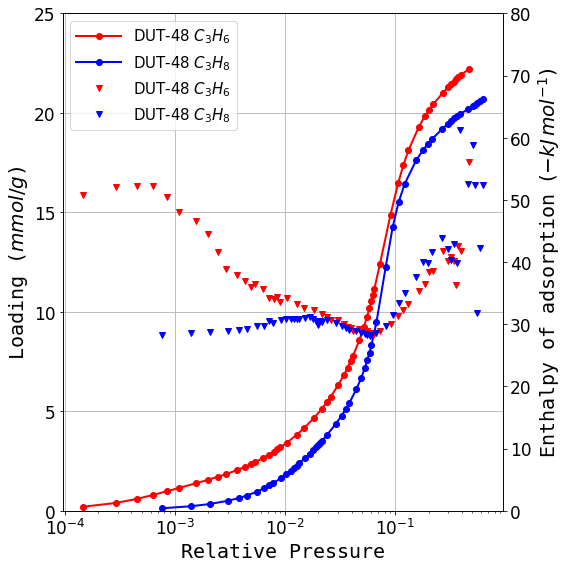
\includegraphics[width=\linewidth]{butane/dut-48-prop-log}%
        \caption{}\label{dut:fgr:dut-48-prop-log}
    \end{subfigure}%
    \begin{subfigure}{0.5\linewidth}
        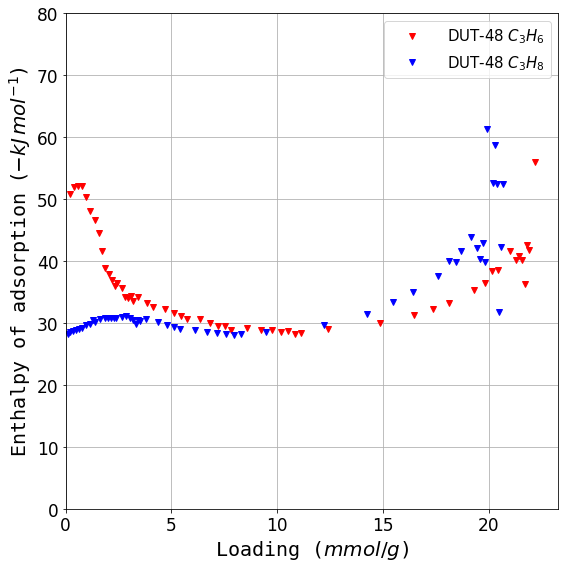
\includegraphics[width=\linewidth]{butane/dut-48-prop-enth}%
        \caption{}\label{dut:fgr:dut-48-prop-enth}
    \end{subfigure}%
    \caption{The (a) isotherms and (b) enthalpy curves of propane 
    and propylene adsorption on DUT-48, highlighting the high energy
    of \ce{C3H6} on specific sites at low pressure, likely to be 
    \(\pi\)-Cu interactions.}%
    \label{dut:fgr:dut-48-prop}
\end{figure}